\chapter{\textbf{\textit{Virtual Microfluidics}}: a hydrogel-based system for simple and robust DNA digital quantification using \textit{in situ} amplification}
This thesis chapter is reproduced from a previously published paper, Xu \textit{et al.}, Nature Methods, 2016 \cite{Xu:2016wt}. Experiments and data analysis were performed by Liyi Xu. 

% \section{Abstract}
% We have developed the hydrogel-based \textit{virtual microfluidics} as a simple and robust alternative to complex engineered microfluidic systems for the compartmentalization of nucleic acid amplification reactions. We applied in-gel digital PCR (dPCR) and in-gel digital multiple displacement amplification (dMDA) to purified DNA templates in the system and demonstrated accurate digital counting of nucleic acid targets. We characterized the dynamic range of the digital amplification and investigated factors controlling the amplification cluster size. We expect \textit{virtual microfluidics} to find application as a low-cost digital assay platform that is highly accessible with an extensive dynamic range. 
%\textit{virtual microfluidics} has the potential to be used as an accessible, versatile low-input DNA analysis tool for various research and clinical applications. 

\section{Introduction}

The absolute quantification of DNA sequences and fragments in genomics \cite{Blainey:2011dt} and prenatal diagnostics \cite{Lo:2007hb} requires assays that enable parallel clonal nucleic acid amplification. DNA quantification by amplification also is needed to overcome nonspecific background for the detection of rare sequence targets in microbial communities and blood-plasma-based diagnostics \cite{Huggett:2015hp,Gevensleben:2013kg,Kuypers:2017it,Johnson:2002wb}.

% Assays involving highly parallel clonal nucleic acid amplification are needed for accurate copy-number analysis with absolute quantification of DNA sequences\cite{Sykes:1992tm,Vogelstain:1999ve} and fragments\cite{Blainey:2011dt} in genomics and prenatal diagnostics\cite{Lo:2007hb}. Such assays are also needed to overcome nonspecific background for the detection of rare sequence targets in microbial communities and blood-plasma-based diagnostics \cite{Huggett:2015hp,Kuypers:2017it,Johnson:2002wb,Gevensleben:2013kg}. 

The traditional method of single-molecule studies requires individual molecules separated in partitions. It is commonly done in engineered microfluidic systems and multi-phase micro-droplet systems, which prevent a broader deployment of digital assays in research labs and in the clinic. Instead of creating physical partitions to isolate individual contents, we decided to build \say{invisible} dividers around them. Passive segregation of single molecules and the product of genome amplification will be able to facilitate genomic analysis of thousands of nucleic acids in parallel. In order to achieve this, a porous structure that is able to fix many molecules and provide a liquid environment for DNA amplification is needed. 

Inspired by earlier work on culturing microbes in hydrogels \cite{Podar:2009ks}, polymerase cloning in polyacrylamide gels using PCR \cite{Mitra:1999ty} and in agarose gels using MDA in conjunction with flow cytometry \cite{Allen:2011jn}, we developed and tested bulk polyethylene glycol (PEG) hydrogels as a general and facile platform for compartmentalizing single molecules and single cells without discrete partitions. This approach, which we call \textit{virtual microfluidics} (Fig. \ref{fig:VM1} and Fig. \ref{fig:GelStructure}), enables massively parallel single-molecule amplification in virtual sub-divisions without the need for engineered micro-devices, multi-phase liquid systems, or instrumentation for cell sorting or microfluidics control. We selected hydrolytically degradable PEG hydrogels that covalently crosslink under mild conditions \cite{Raeber:2005cq}. The chemically selective crosslinking reaction used in our method does not damage templates or inhibit subsequent reactions and forms gels that are stable to high temperatures. The mesh size of the PEG gel allows diffusion of small molecules, oligonucleotides, and enzymes but immobilizes cells and high-molecular-weight nucleic acids \cite{Wu:2009ez}. If desired, PEG gels can be functionalized to selectively immobilize low molecular weight species by attachment to the gel matrix \cite{Phelps:2011dka}.

\begin{figure} 
\centering
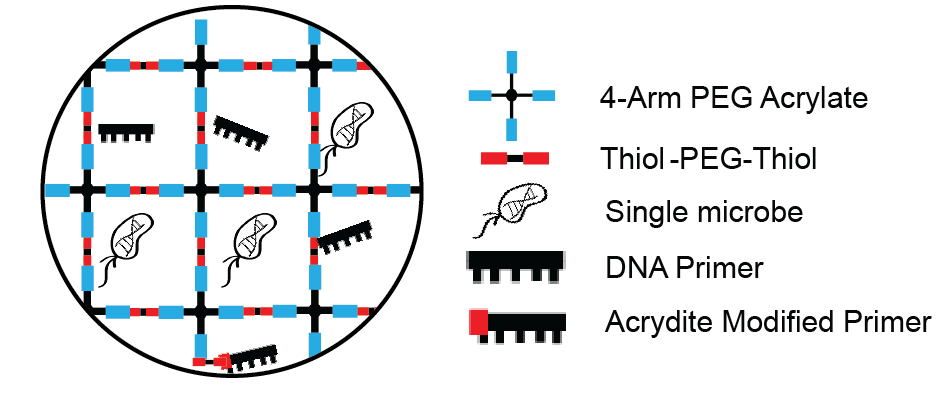
\includegraphics[keepaspectratio,width=0.6\textwidth]{./figures/SolidPhaseWGA-21}
\caption[The \textit{virtual microfluidics} hydrogel structure.]{The \textit{virtual microfluidics} hydrogel structure (not to scale).}
\label{fig:GelStructure}
\end{figure}

Hydrogels are formed by crosslinking polymer chains through physical, ionic or covalent interactions and are best known for their ability to absorb water \cite{Elisseeff:2008cm}, which makes them an ideal candidate for solid-phase DNA amplification. Note that solid-phase here means in-gel, compared to liquid-phase reactions. Previously, the polyacrylamide hydrogel has been used as a scaffold for solid-phase DNA amplification \cite{Mitra:1999ty}. However, polyacrylamide gel crosslinks with the free radicals initially produced by ammonium persulfate or by photochemical polymerization. The free radicals have been found to inhibit reverse-transcription PCR and inhibit DNA dyes such as SYBR Green and LC Green plus \cite{Atrazhev:2010ex} for real-time monitoring, while photochemical polymerization might introduce DNA damage to the target of interest. Such DNA oxidative stress caused by the addition of free radicals is a pervasive cause of sequencing error and directly confound variant identification \cite{Chen:2017dq}. Luckily, a new generation of PEG-based multi-arm hydrogel has been developed that provide many advantages for our purpose \cite{Tan:2010by}. Specifically, 4-arm PEG hydrogel with various end moieties has been applied for gene delivery and to bulid 3D scaffolds for tissue engineering. The hydrogels are formed via Michael addition chemistry by reacting a 4-arm acrylate terminated PEG with a thiol-functionalized PEG \cite{Li:2012bd}. The use of Michael addition chemistry allows for \textit{in situ} hydrogel formation under physiological conditions, which will cause minimal damage to the DNA and cells of interest in broad applications. In addition, while acrylamide powder is neurotoxic, 4-arm PEG components pose no such harm to researchers. In terms of mesh size, Raeber \textit{et al.} and Kraehenbuehl \textit{et al.} have shown that 4-arm PEG's pore size is between 25 nm and 100 nm depending on the weight percentage \cite{Raeber:2005cq,Kraehenbuehl:2008do}.


Two types of DNA amplification---PCR and MDA are characterized for digital quantlification. PCR amplifies sequence specific region locally defined by forward and reverse primers, while MDA amplifies the template DNA globally through random primer binding. In this chapter, I descrbied the characterization on both amplification methods and focused on MDA method because of its wide application in enabling low-input genomics. 


\section{Results and Discussion}
\subsection{Digital PCR in-gel characterization}

\begin{figure} 
\centering
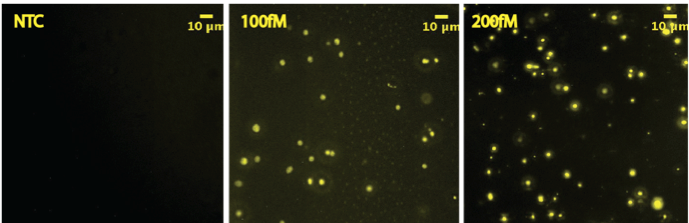
\includegraphics[keepaspectratio,width=0.6\textwidth]{./figures/dPCR_Capillary.png}
\caption[DNA amplification clusters from PCR in hydrogel in capillary tubes.]{DNA amplification clusters from PCR in hydrogel in capillary tubes. Images are taking using a Nikon wide-field fluorescent microscope. The concentration of DNA template was labeled in units of femtomolar (fM). The capillary tube is 50 $\mu$m tall. Scale bars represent 10 $\mu$m.}
\label{fig:dPCR_Cap}
\end{figure}

In order to characterize \textit{virtual microfluidics}, purified lambda phage DNA is used as the template to conduct DNA amplification in the PEG hydrogel. \textlambda DNA is a common, well-characterized substrate for restriction endonucleases and its sequence and properties have been well-understood \cite{Fu:2011wc, Robertson:2006gi}. The 48502 bp length acts as a useful proxy for genomic DNA from bacteria or mammalian cells. In order to quantify the robustness of solid phase DNA amplification and estimate the dynamic range of the technology, a range of DNA template concentrations from serial dilutions of a stock were used. Reaction components consisting of 4-arm PEG-acrylate, dithiol-PEG, PCR reaction buffer, primers, dNTP, DNA polymerase and template are mixed thoroughly before loaded in a reaction chamber. Various experimental configurations such as PDMS channels, capillary glass tubes (Fig. \ref{fig:dPCR_Cap}), thin PDMS wells (10 $\mu$m to 50 $\mu$m), and frame-seal chambers (Biorad) have been tested, with the frame-seal chamber (Fig. \ref{fig:FigAbstract} in Chapter 1 and Fig. \ref{fig:dPCR_FS} in methods) proved to be the most efficient and consistent loading method. Several types of DNA polymerase with different levels of fidelity, 3'-5' proofreading, and primer extension capacity, such as Jumpstart \textit{Taq}, Vent (exo-), Vent, have been tested in hydrogel for amplification optimization. Fig. \ref{fig:dPCR_Calibration} indicates that accurate digital counting was achieved by PCR in gel. 

\subsection{Digital MDA in-gel characterization}
In addition to PCR in hydrogel, Multiple Displacement Amplification (MDA) is conducted for whole genome amplification in hydrogel. MDA \cite{Dean:2002us} is a popular amplification method for single-cell genome sequencing \cite{Marcy:2007il,Fu:2015gl,Zhang:2006hq,Raghunathan:2005fg,Pamp:2012cj,Dodsworth:2013ih,Hess:2011gu}. To evaluate the \textit{virtual microfluidics} concept for WGA, we tested dMDA \cite{Morinishi:2015jx,Blainey:2011dt} of purified, diluted Lambda phage DNA in the hydrogel format (Fig. \ref{fig:dMDA}a-c, Fig. \ref{fig:dMDA_Quant} and Methods). Our estimate of 10 pg MDA product per cluster (Fig. \ref{fig:dMDA_MammalianEcoliCluster}) suggests that we approached endpoint product concentrations typical of conventional liquid MDA reactions (\ensuremath{\sim}800 ng\slash $\mu$L) \cite{Blainey:2013dp}. We varied parameters to test how \textit{in situ} single-molecule MDA reactions can be controlled (Fig. \ref{fig:dMDA} and Fig. \ref{fig:dMDA_Quant}), observing that the smaller pore sizes in higher density gels limit the spread of DNA products.

\begin{figure}
\centering
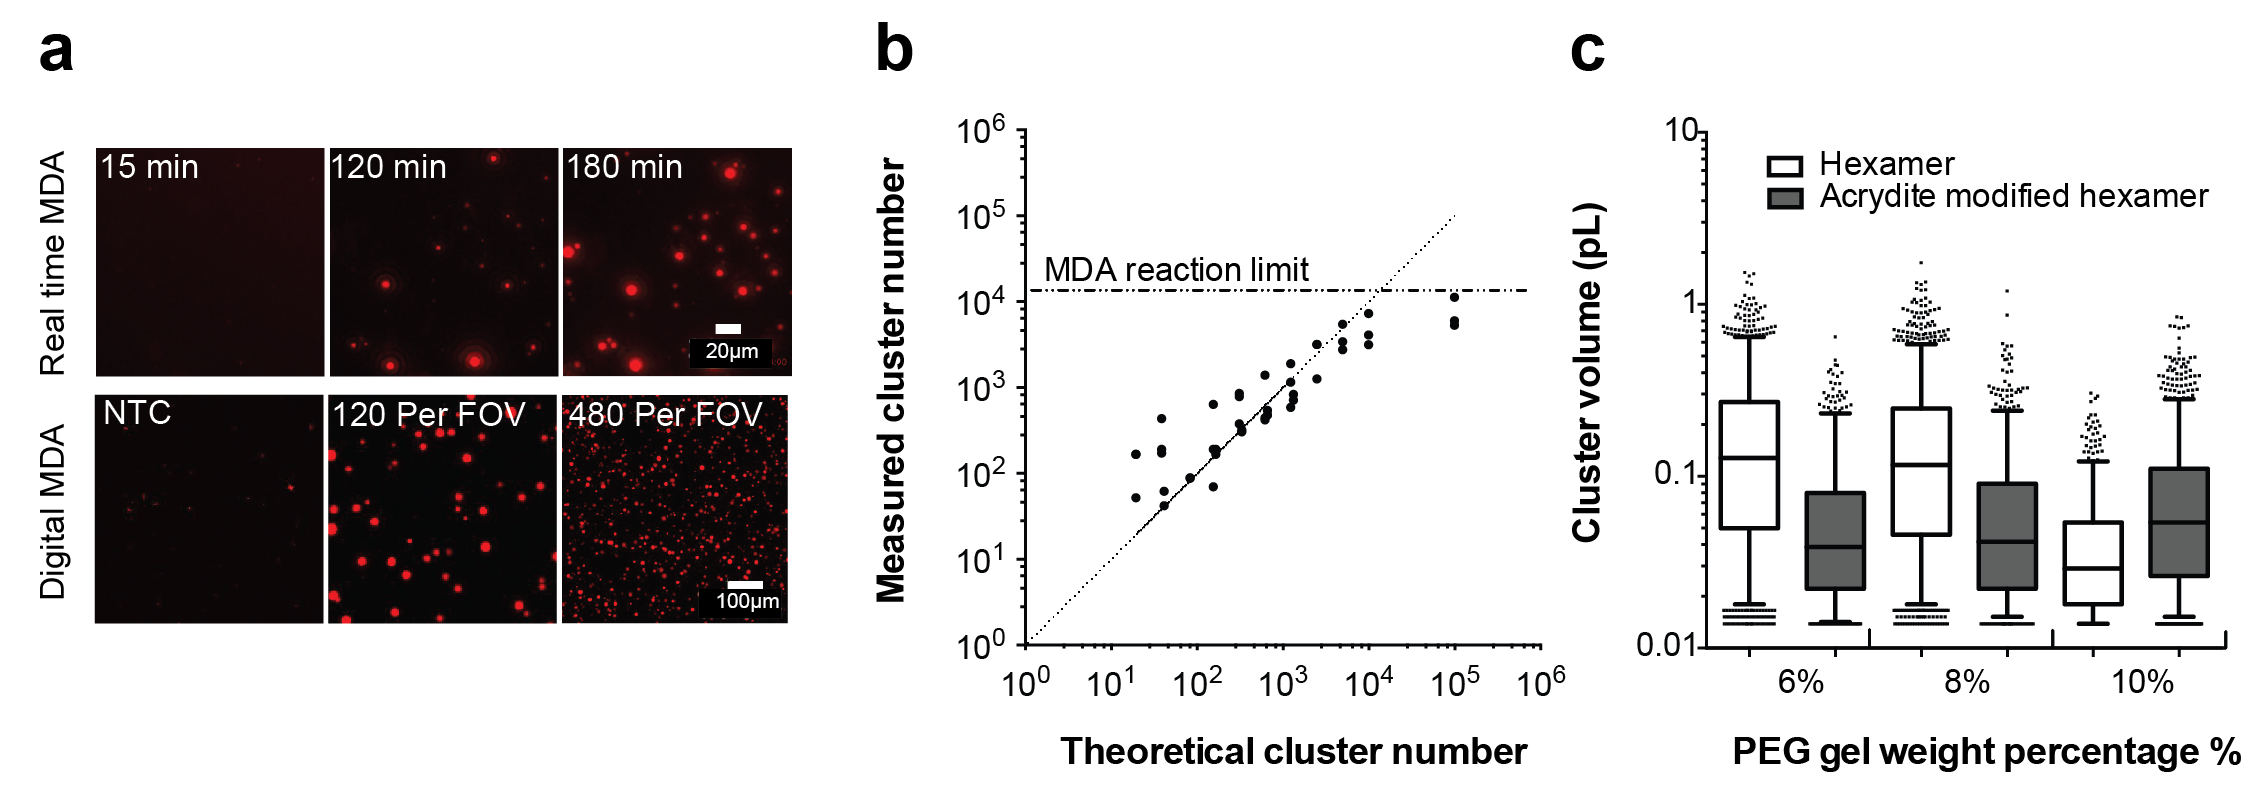
\includegraphics[keepaspectratio,width=1\textwidth]{./figures/Thesis-21.png}
\caption[Digital single-molecule MDA in hydrogel (Lambda phage DNA).]{Digital single-molecule MDA in hydrogel (Lambda phage DNA).(a) Real-time and digital MDA in PEG hydrogel. Top, time-lapse
epi-fluorescence images (SYTOX Orange DNA stain) illustrate MDA cluster growth from individual template molecules. Bottom, DNA cluster number increases with template concentration. FOV, 650 nm $\times$ 650 nm field of view. NTC, no DNA template control. (b) Calibration curve illustrates linear relationship between template concentration and cluster number (n = 2 or 3 FOV at
each concentration). (c) MDA cluster size is correlated with gel weight percentage and affected by acrydite-modified hexamer anchorage. Data is shown as 5$\%$ {\textendash} 95$\%$ box plots with scattered outliers and center line for median. (n = 1334, 1587, 684, 704, 869 and 1301).}
\label{fig:dMDA}
\end{figure}

A similar sample preparation and loading method are used for dMDA compared to dPCR in the hydrogel. The only difference for dMDA in the hydrogel is the UV decontamination step on all reaction components except the polymerase. A study by Woyke \textit{et al.} has shown that the calibrated UV decontamination step can effectively remove contaminant DNA without introducing significant coverage biases or variants \cite{Woyke:2011eg}. 

\begin{figure}
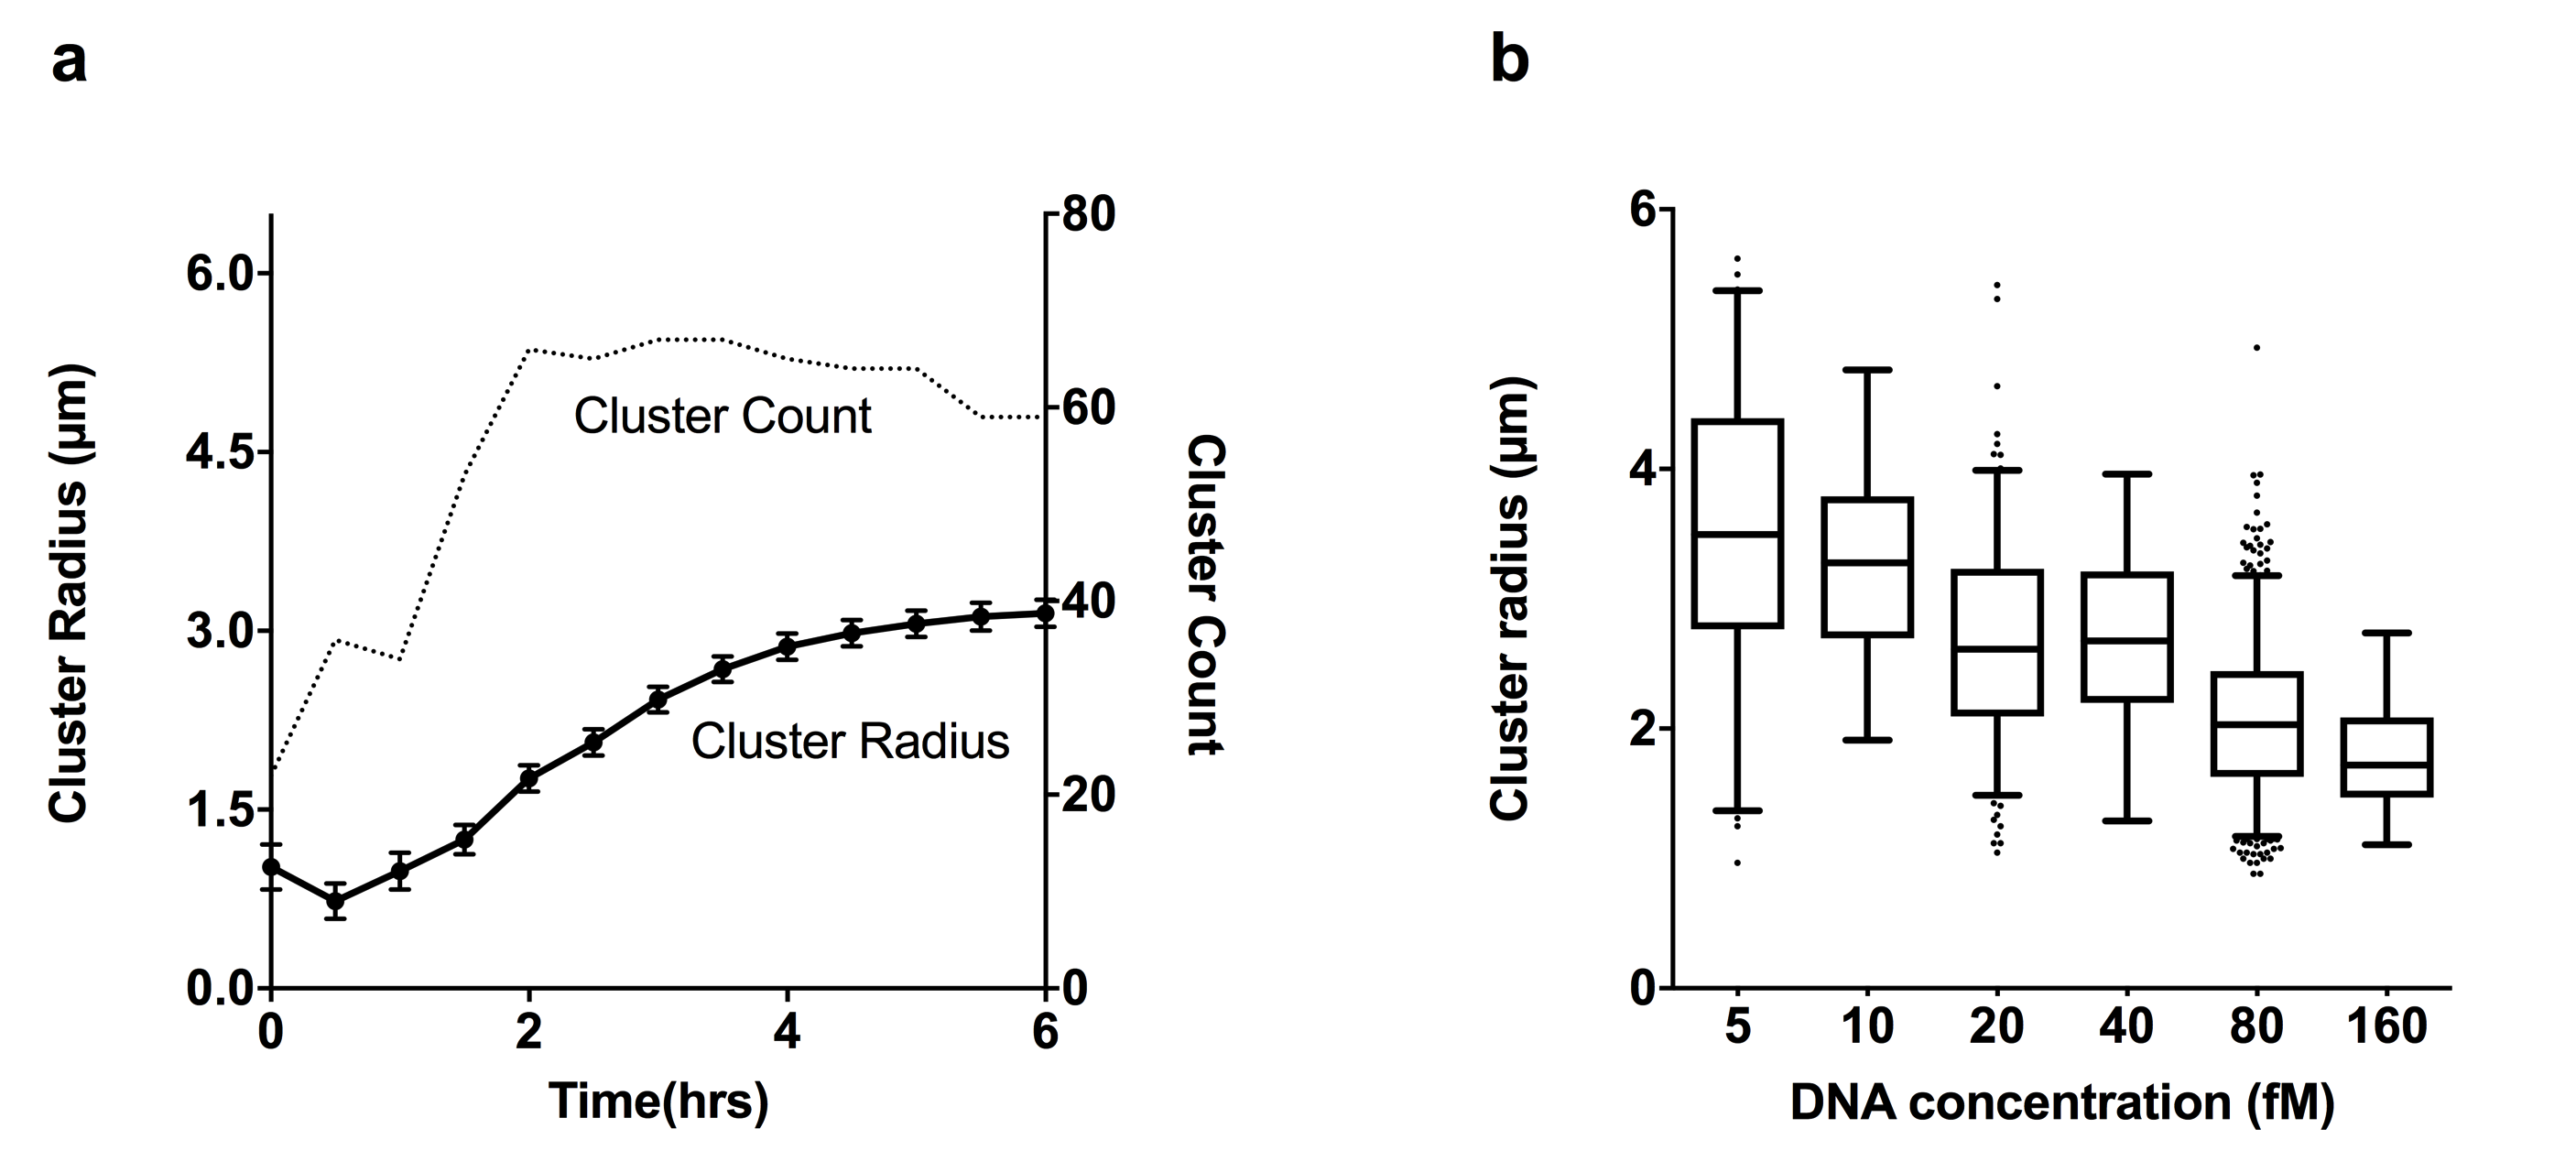
\includegraphics[keepaspectratio,width=1\textwidth]{./figures/Supp1_4.png}
\caption[Real time dMDA and MDA cluster size]{Real time dMDA and MDA cluster size. (a) Real time digital MDA for quantification of cluster growth (mean radius $\pm$ SEM) and count with time. The zero time point cluster count and radius data points reflect the properties of fluorescent contaminants. (b) MDA cluster size decreases with increasing DNA template concentration with the same gel condition. Data is shown as 5$\%$ {\textendash} 95$\%$ box plot with outliers scattered and the centerline as the median. (n = 2 fields of view at each concentration, number of clusters for each field of view is: n = 43, 62, 89, 88, 191, 167, 321, 305, 478, 542, 711, 833).}
\label{fig:dMDA_Quant}
\end{figure}

With the success of dPCR and dMDA in the hydrogel, a robust but straightforward image analysis method is needed to obtain the absolute count of DNA molecules and the size of DNA amplification clusters. Currently, image analysis is conducted on the raw confocal stacks using the Fiji Image J. The Image J particle analyzer plug-in is widely used for counting particles and cells. Confocal stacks were taken with consistent laser power and integrated with a Z intensity gradient to minimize cluster fluorescent saturation. Each gel stack, roughly 300 $\mu$m thick, was first projected in Z direction with the maximum intensity for a faster 2D processing. Then, a thresholding algorithm is chosen manually based on the visual comparison between the original projection and the thresholded image. This image analysis method has been proved effective in measuring the number and the size of DNA amplification clusters. However, a more consistent and robust image analysis routine might be needed for a higher-sensitivity application. 

\subsection{DNA amplification cluster analysis}
Understanding the mechanism of cluster growth and effectively controlling the size of the end product are keys ensuring the broader applicability of this technology. Key parameters include initial DNA concentration, hydrogel weight percentage, primer modification chemistry and amplification time. One hypothesis regarding the size of clusters is that with a higher PEG hydrogel weight percentage, tighter clusters should be generated. Higher PEG weight percentage means more 4-arm PEG acrylate and dithiol-PEG in a fixed volume. Thus, the hydrogel network will provide a smaller mesh size for DNA template and prevent amplification product from moving further due to restricted diffusion. Another possibility is that a tighter mesh size might compromise the robustness of DNA amplification reaction due to the physical impedance. 

Another way to control the DNA amplification cluster size could be to add a chemical moiety to the primers. Acrydite modification on DNA probes has been used frequently to attach primers to various hydrogel platforms \cite{Mitra:1999ty}. In this case, acrydite reacts with the part of the thiol groups on dithiol-PEG and unreacted thiol groups will crosslink with 4-arm PEG acrylate. Varying the modified primers' concentration and its ratio to standard primer concentration gave us new insights on how to control cluster size (Fig. \ref{fig:dMDA}c). 

Meanwhile, real-time monitoring on the DNA clusters' growing helps determine the optimal reaction time and cycle numbers for both MDA and PCR reactions (Fig. \ref{fig:dMDA_Quant}a). It will be also useful to help decide on a cut-off reading time to prevent false-positive readings including the small primer-dimer clusters and clusters from short DNA fragments mixed in a genomic DNA sample (Fig. \ref{fig:dMDA_Quant}a).

\subsection{Dynamic range of in-gel digital MDA}
When the input for digital MDA is very low (fewer than 100 per field of view), molecular counts are significantly inflated by contaminating fluorescence signals (contaminating DNA fragments or particles) that are not differentiated from true counts by our image analysis algorithm. At high target concentrations, the DNA clusters crowd one another, limiting the maximum useful concentration to 10,000 DNA molecules per field of view. For MDA, the smaller cluster sizes observed at higher template concentration (Fig. \ref{fig:dMDA_Quant}b) benefit assay dynamic range by improving cluster identifiability at the highest template concentrations. Based on our estimate of 10 pg DNA per cluster (Fig. \ref{fig:dMDA_MammalianEcoliCluster}), 10,000 - 100,000 clusters per field of view in our setup approximates typical maximum product concentrations of about 800 ng\slash $\mu$L achieved in conventional liquid MDA reactions. The assay dynamic range can be improved by manipulating the DNA cluster size, increasing the volume of gel imaged (e.g. by combining multiple fields of view), improving image processing methods, and further reducing the number of fluorescent contaminants. 

\begin{figure}
\centering
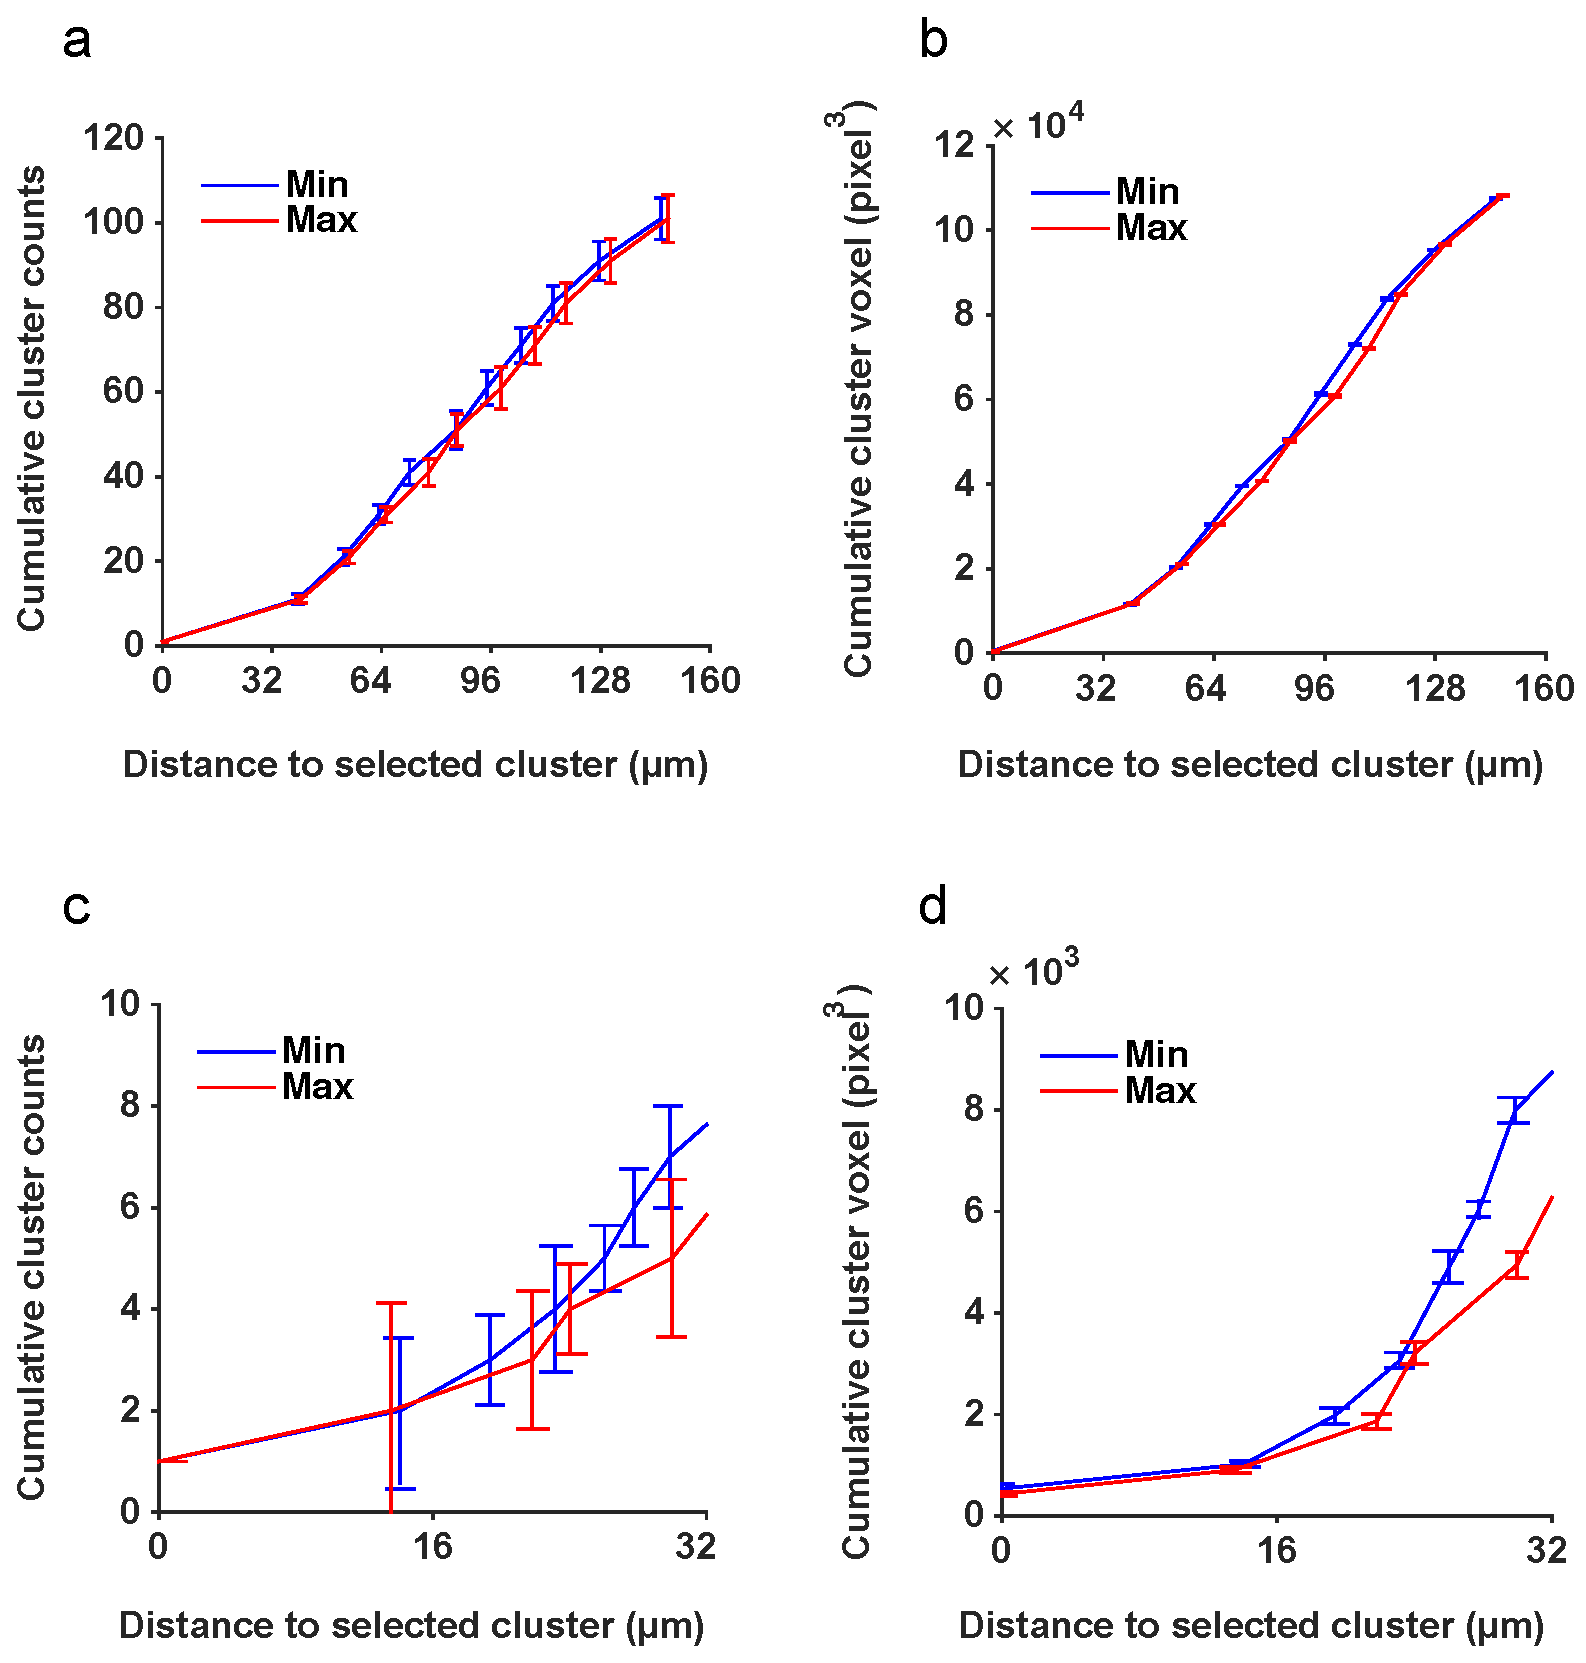
\includegraphics[keepaspectratio,width=0.8\textwidth]{./figures/10fM001_5ClusterZoomOut}
\caption[Cluster size and location correlation analysis]{Cluster size and location correlation analysis. Five reference clusters with the largest radii and five reference clusters with the smallest radii were chosen among clusters in one field of view (100+ clusters) of one MDA hydrogel sample. a) By zooming out from selected clusters, the number of other clusters encountered at successively greater distances was plotted. b) The total volume of other clusters encountered was plotted. c) and d) are zoom-in views of a) and b) at 0 to 32 $\mu$m from reference clusters. We hypothesized that large clusters consume local resources and thus, would reduce the number and/or size of surrounding clusters. Although slight enhancements in the number and size of clusters surrounding the set of small reference clusters versus the set of large reference clusters exist, the effect is small. Error bars are SEM.}
\label{fig:ClusterCorrelation}
\end{figure}

\subsection{Analysis of reaction extent limitation and local competition among MDA clusters}
Based on Fig. \ref{fig:ClusterCorrelation}, we concluded that a global auto-inhibition mechanism limits the growth of MDA clusters. We analyzed the variability in cluster number and DNA content around large and small reference clusters to test for local reagent competition among WGA reaction centers, finding little evidence for local competition. This observation is consistent with the high diffusion constants for enzymes, primers, and nucleotides measured in PEG hydrogels similar to ours \cite{Wu:2009ez,Weber:2009fe}. No specific limiting reagent was identified when reactants were supplemented individually (data not shown). The final reaction pH in our hydrogel reactions was measured to be 6.5 (initial pH = 7.5), which may limit cluster growth due to a global loss of polymerase activity at lower pH. Altogether, these data are consistent with density-dependent average size variation by global auto-inhibition, possibly by the pH drop. Variability of cluster size in a single experiment may result from variable initial template conformation, the degree of template denaturation, or local inhomogeneities in the hydrogel structure.

\section{Conclusion}
Here we tested the performance of \textit{virtual microfluidics} in-gel digital PCR and digital MDA amplification as an analytical method for molecular counting assays. \textit{Virtual microfluidics} enables high-throughput digital assays and preparative whole-genome amplification without microfabricated consumables or expensive instrumentation. Up to 20,000,000 analytes per $\mu$L could be accommodated due to the nature of the diffusion-restricted reaction and the continuous virtual chambers. Throughput could be increased by using a thinner gel with more surface area. Its excellent optical accessibility allows potential fluorescent labeling of rare sequences, which is a key in identifying rare targets in liquid biopsy applications. We expect \textit{virtual microfluidics} to find applications as low-cost, highly accessible digital assay platforms that offer superior sensitivity and dynamic range. 

% The solid phase amplification environment also can contain potential infectious targets to minimize the handling of biohazardous materials for infectious disease diagnosis in the clinic and at the point-of-care diagnostic setting.

\section{Materials and Methods}
\subsection{PEG hydrogel cross-linking}
Hydrogel components, including 4-arm PEG acrylate (MW 10,000) and HS-PEG-SH (MW 3,400), were obtained from Laysan Bio. For every 25 $\mu$L of 10\% (wt\slash v) cross-linked hydrogel, 1.6 mg of 4-arm PEG acrylate and 1.1 mg of HS-PEG-SH were dissolved in pH 7.4 PBS (Invitrogen). It was briefly vortexed and centrifuged to ensure mixing and it was allowed to sit on the bench for 10 min while the hydrogel components cross-linked through the reaction between the thiol and acrylate groups.
\subsection{In-gel digital PCR}
The primers (Table \ref{tab:ESprimerList}) used for PCR on purified \textlambda DNA (48 kbp, NEB) were ordered through IDT(Integrated DNA Technologies). A 25 $\mu$L hydrogel PCR reaction consisted of 2 U of VentR (exo-) polymerase (NEB), 1$\times$ ThermoPol Reaction Buffer (NEB), 0.4 mM dNTP (NEB), 1 $\mu$m Primers, 5\% DMSO (Sigma), 0.5 mg\slash mL BSA (NEB), 1.6 mg 4-arm PEG acrylate in PBS, 1.1 mg HS-PEG-SH in PBS, and \textlambda DNA template (NEB) of various concentrations. The 25 $\mu$L above components were loaded in a 9 mm by 9 mm frame-seal chamber (Bio-rad). The following thermal protocol was ran on an MJ Research PTC--100 twin tower thermal cycler: 30 $^{\circ}$C for 30 min (gel polymerization), 98 $^{\circ}$C for 3 min; 98 $^{\circ}$C for 30 sec, 57 $^{\circ}$C for 30 sec, 72 $^{\circ}$C for 1 min for 40 to 60 cycles; 72 $^{\circ}$C for 5 min and hold at 4 $^{\circ}$C. The gel was stained with 500 nM SYTOX Orange nucleic acid dye (Invitrogen) (Fig. \ref{fig:dPCR_FS} and \ref{fig:dPCR_Calibration}).

\begin{figure}
\centering
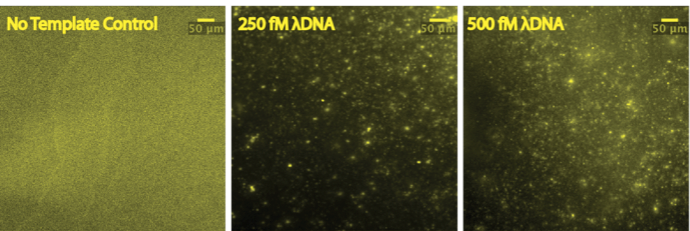
\includegraphics[keepaspectratio,width=0.6\textwidth]{./figures/dPCR_FrameSeal.png}
\caption[DNA amplification clusters from PCR in frame-seal chambers.]{DNA amplification clusters from PCR in hydrogel in frame-seal chambers. Each image is a z-axis max projection from a confocal tiff stack taken by a Zeiss spinning disk confocal microscope. Scale bars represent 50 $\mu$m.}
\label{fig:dPCR_FS}
\end{figure}

\begin{figure}
\centering
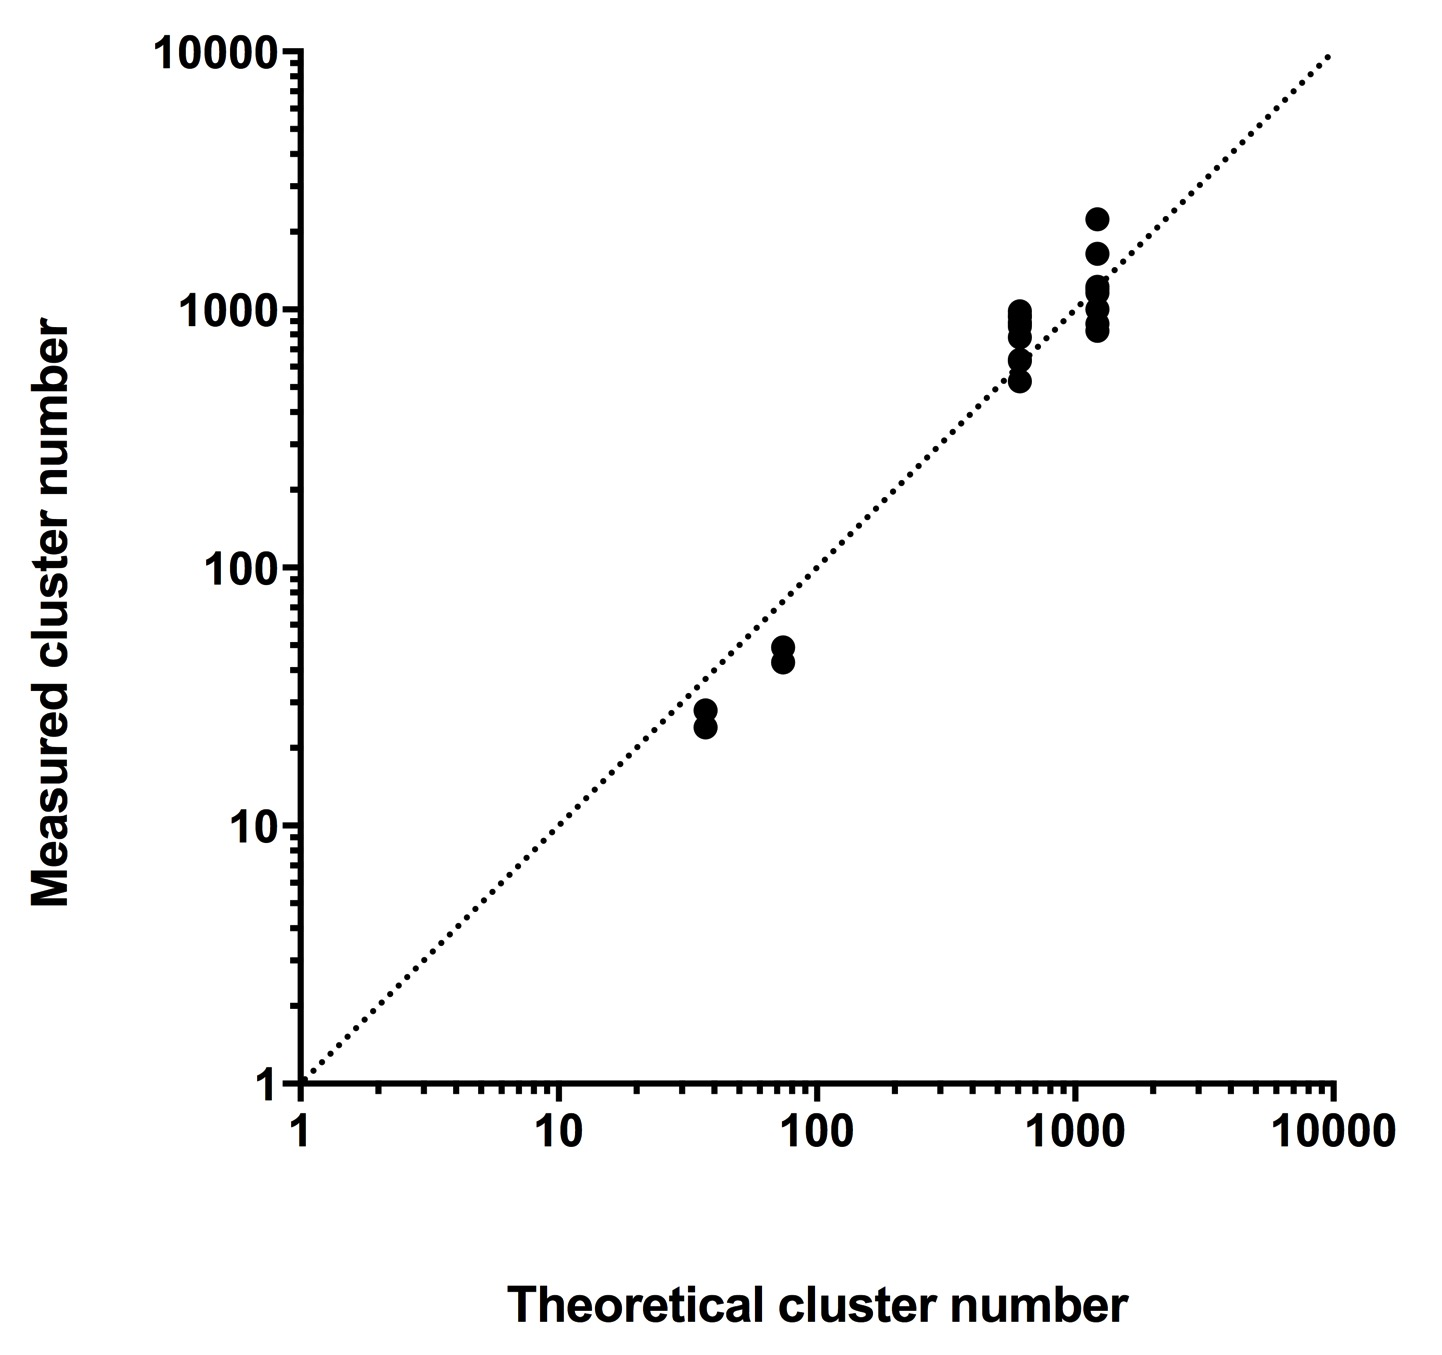
\includegraphics[keepaspectratio,width=0.5\textwidth]{./figures/SuppFig3.jpg}
\caption[Digital single-molecule PCR in hydrogel (Lambda phage DNA).]{Digital single-molecule PCR in hydrogel (Lambda phage DNA). Measured cluster number per field of view versus calculated cluster number based on template concentration. Reaction conditions are described in methods (PCR). The dotted line indicates the ideal situation when measured cluster number equals to the theoretical cluster number.}
\label{fig:dPCR_Calibration}
\end{figure}

\subsection{In-gel digital MDA}
A 25 $\mu$L hydrogel MDA reaction consisted of 0.5 $\mu$L of REPLI-g sc Polymerase (Qiagen), 1$\times$ $\Phi$29 buffer (NEB), 50 $\mu$m random hexamers (IDT; including two phosphorothioate bonds at 3' terminus), 2.5\% DMSO, 0.4 mM dNTP, 0.5 mg\slash mL BSA, 500 nM SYTOX Orange (Invitrogen) and denatured \textlambda DNA. \textlambda DNA was denatured using alkaline buffer ``D1'' (Qiagen) and neutralized using buffer ``N1''(Qiagen) according to Qiagen REPLI-G sc kit protocol prior to hydrogel encapsulation. All MDA and gel components, except polymerase and SYTOX Orange dye, were UV treated for 30 min using the Stratalinker UV crosslinking instrument (Stratagene) to render contaminating background DNA incompetent for MDA. The 25 $\mu$L reaction mixture was loaded in a 9 mm by 9 mm frame-seal chamber (Bio-rad, about 300 $\mu$m in height). The gel was sealed in the chamber with a plastic cover and maintained at 30 $^{\circ}$C for 8 hours or longer in the MJ Research PTC--100 twin tower thermal cycler. After the reaction, we imaged the gel using Nikon ECLIPSE Ti inverted microscope or Nikon ultra-fast laser scanning confocal microscope (MIT Koch Institute Microscopy Core Facility) (Fig. \ref{fig:dMDA_Quant}a).
\subsection{In-gel real-time dMDA}
MDA hydrogel reactions were set up as described above and conducted at room temperature for 6 hours on a Nikon ECLIPSE Ti Epi-Fluorescence Microscope excited with a Lumencor Spectra X light engine (Lumencor) with fluorescent emissions filtered through a SpGold filter (Semrock) (Fig. \ref{fig:dMDA_Quant}b). MATLAB was used to capture time-lapse image stacks through a Nikon 20$\times$\slash 0.4 NA objective and Hamamatsu C11440 camera with 15 min intervals, 100 ms exposure time, and 10\% Lumencor excitation power. All samples were stained with 500 nM SYTOX Orange. Each \textit{E. coli.} MDA cluster or mammalian cell image stack was cropped and processed as described below.


% \begin{figure}
% \centering
% 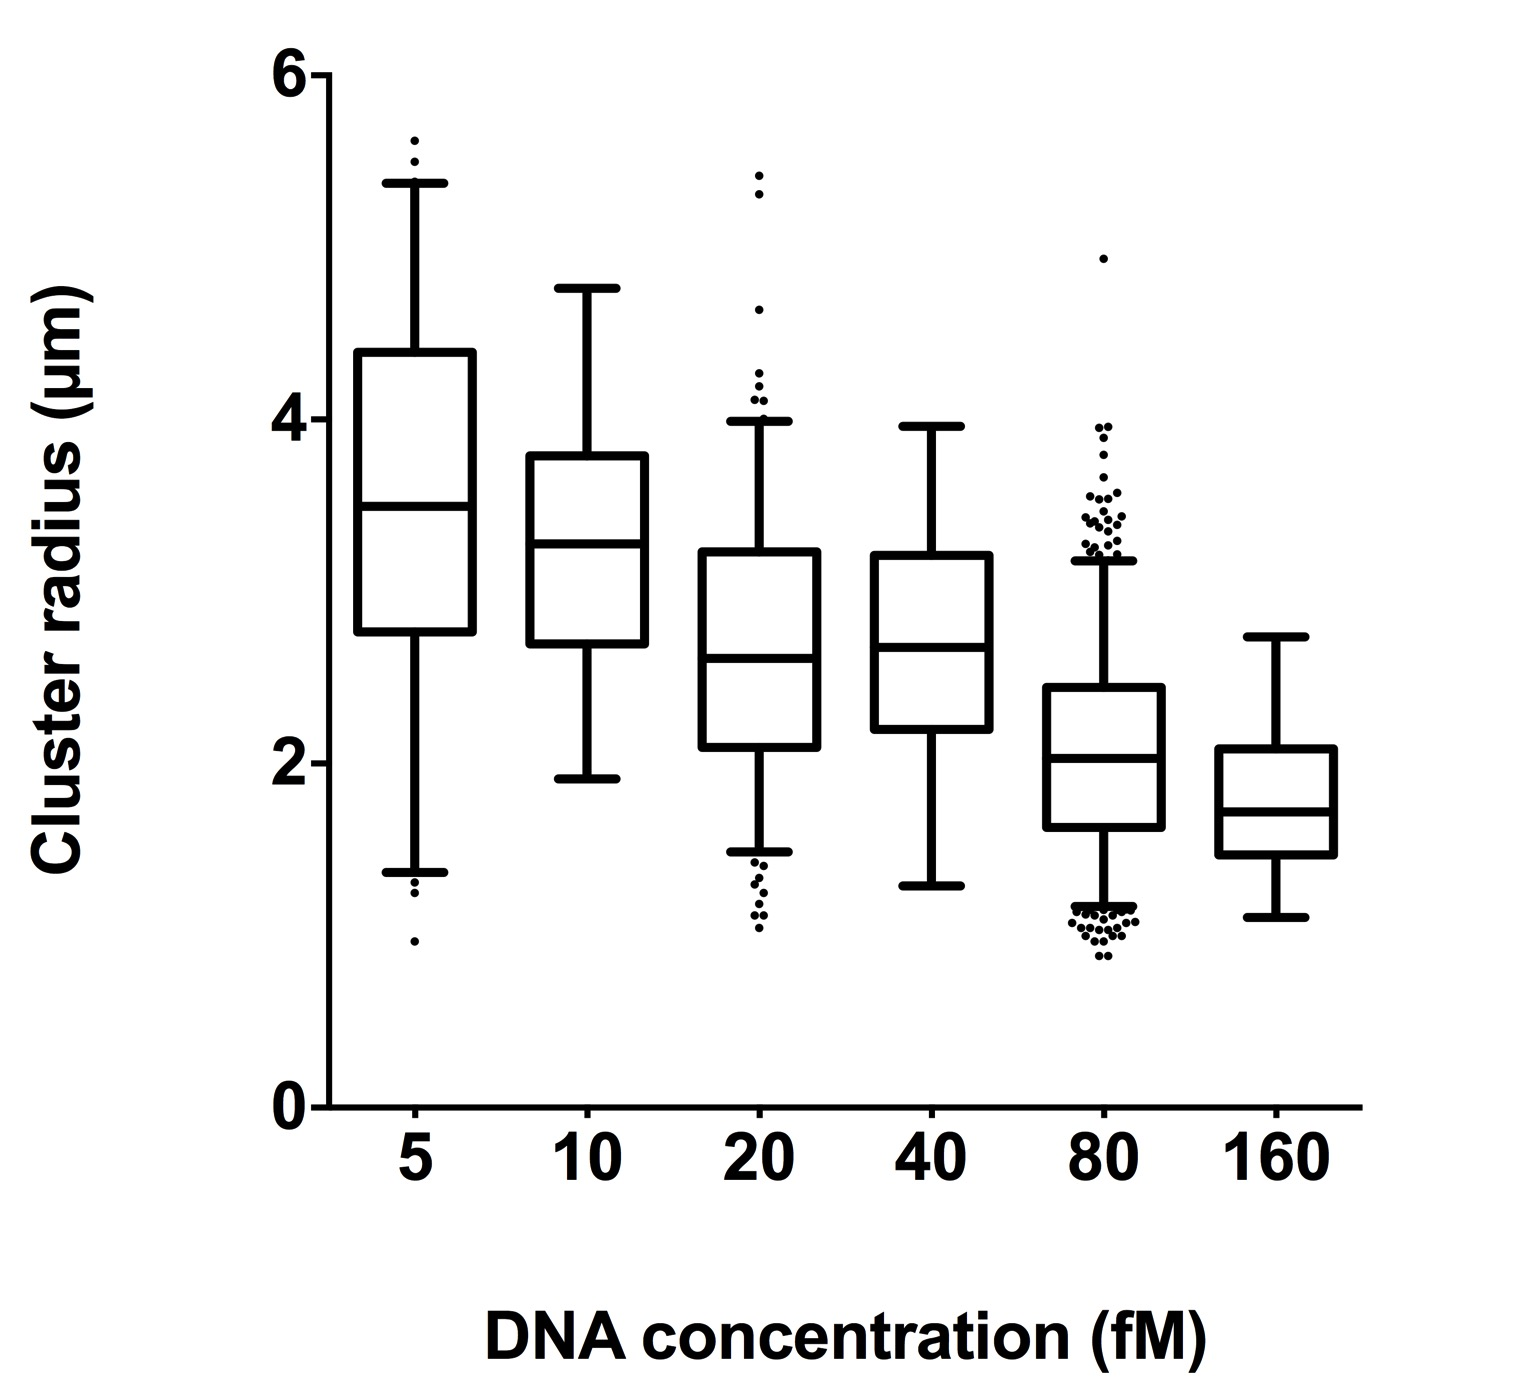
\includegraphics[keepaspectratio,width=0.5\textwidth]{./figures/SuppFig4.jpg}
% \caption[MDA cluster size decreases with increasing DNA template concentration]{MDA cluster size decreases with increasing DNA template concentration with the same gel condition. Data is shown as 5 \% - 95 \% box plot with outliers scattered and the centerline as the median. (n = 2 fields of view at each concentration, number of clusters for each field of view is: n = 43, 62, 89, 88, 191, 167, 321, 305, 478, 542, 711, 833).}
% \label{fig:dMDA_Quant}
% \end{figure}

% \begin{figure}
% \centering
% 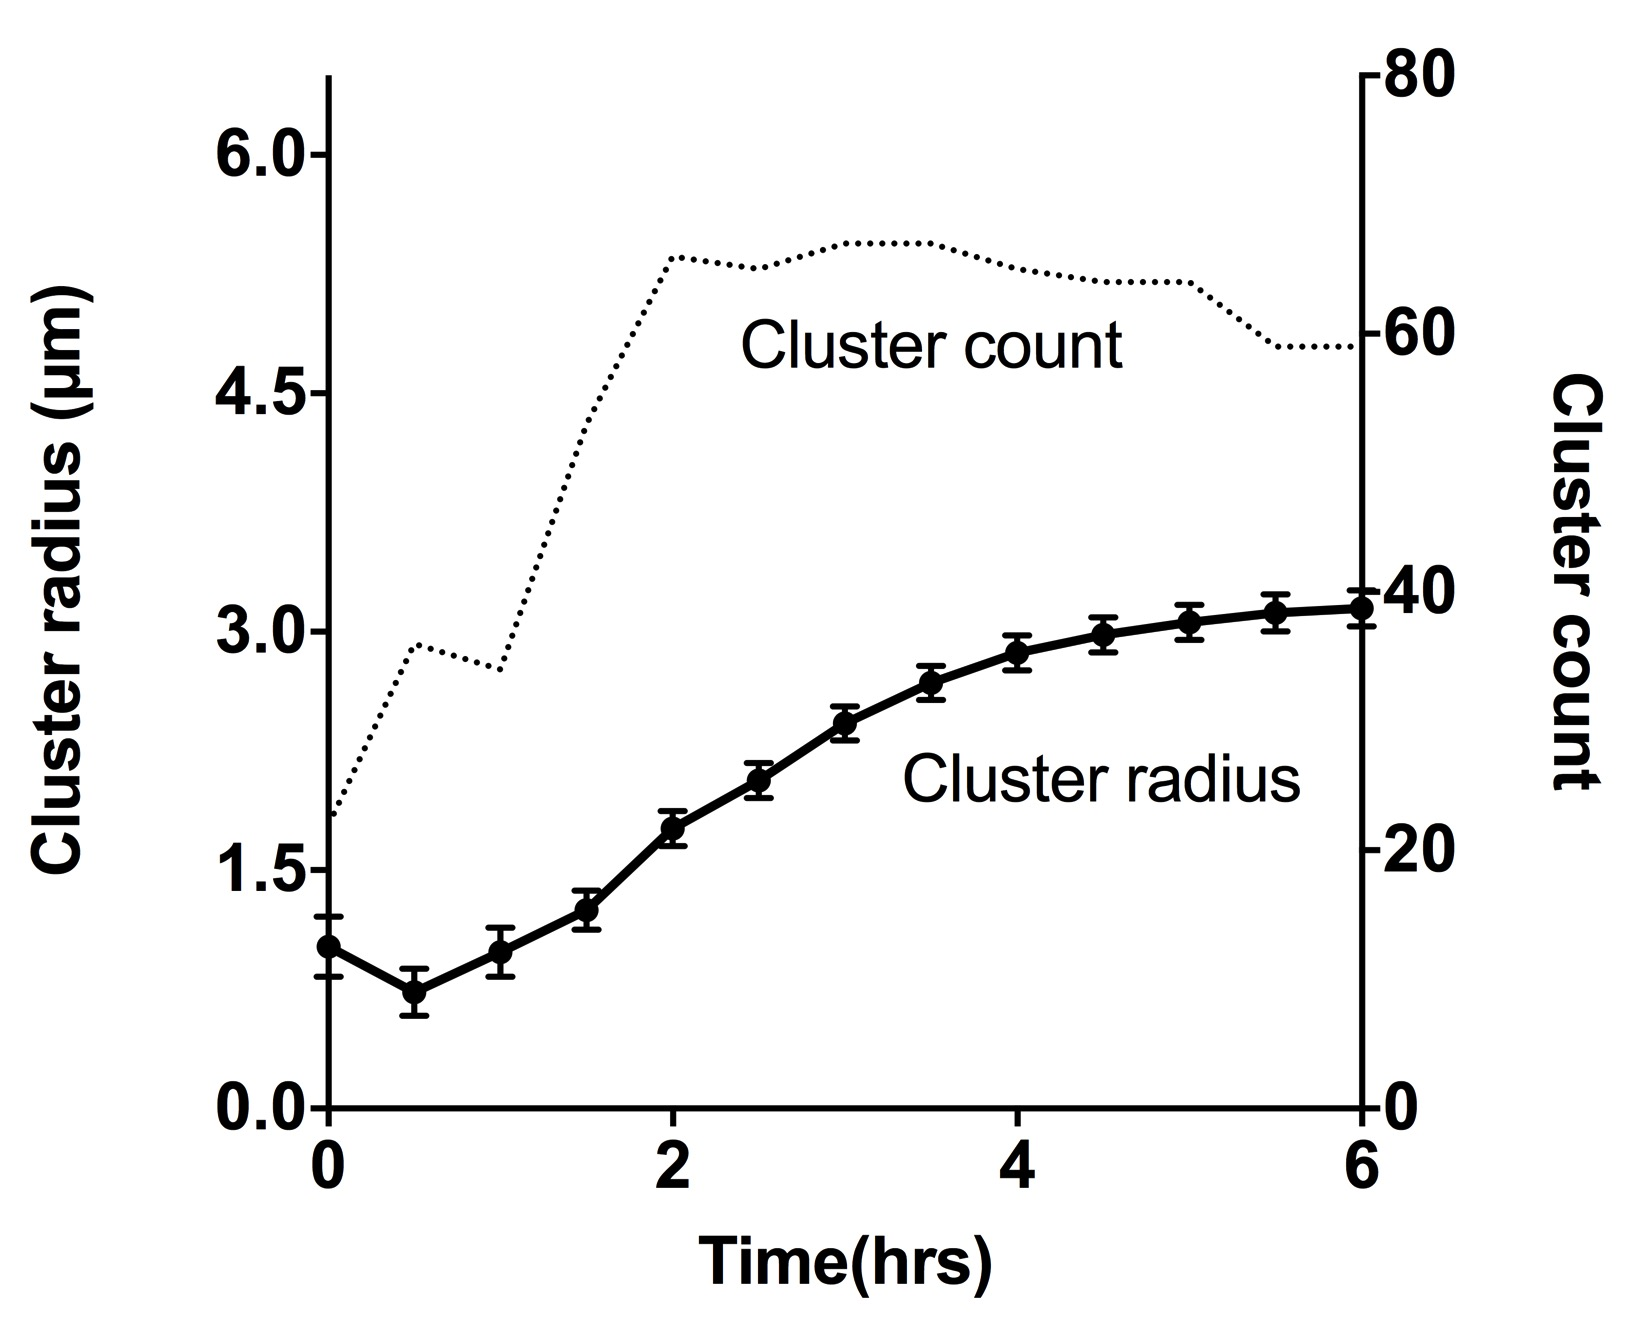
\includegraphics[keepaspectratio,width=0.5\textwidth]{./figures/SuppFig1.jpg}
% \caption[Real time dMDA for quantification of cluster growth and count with time.]{Real time dMDA for quantification of cluster growth and count with time. The cluster radius curve shows mean radius $\pm$ SEM. The zero time point cluster count and radius data points reflect the properties of fluorescent contaminants.}
% \label{fig:dMDA_Quanttime}
% \end{figure}

% \begin{figure}
% \centering
% 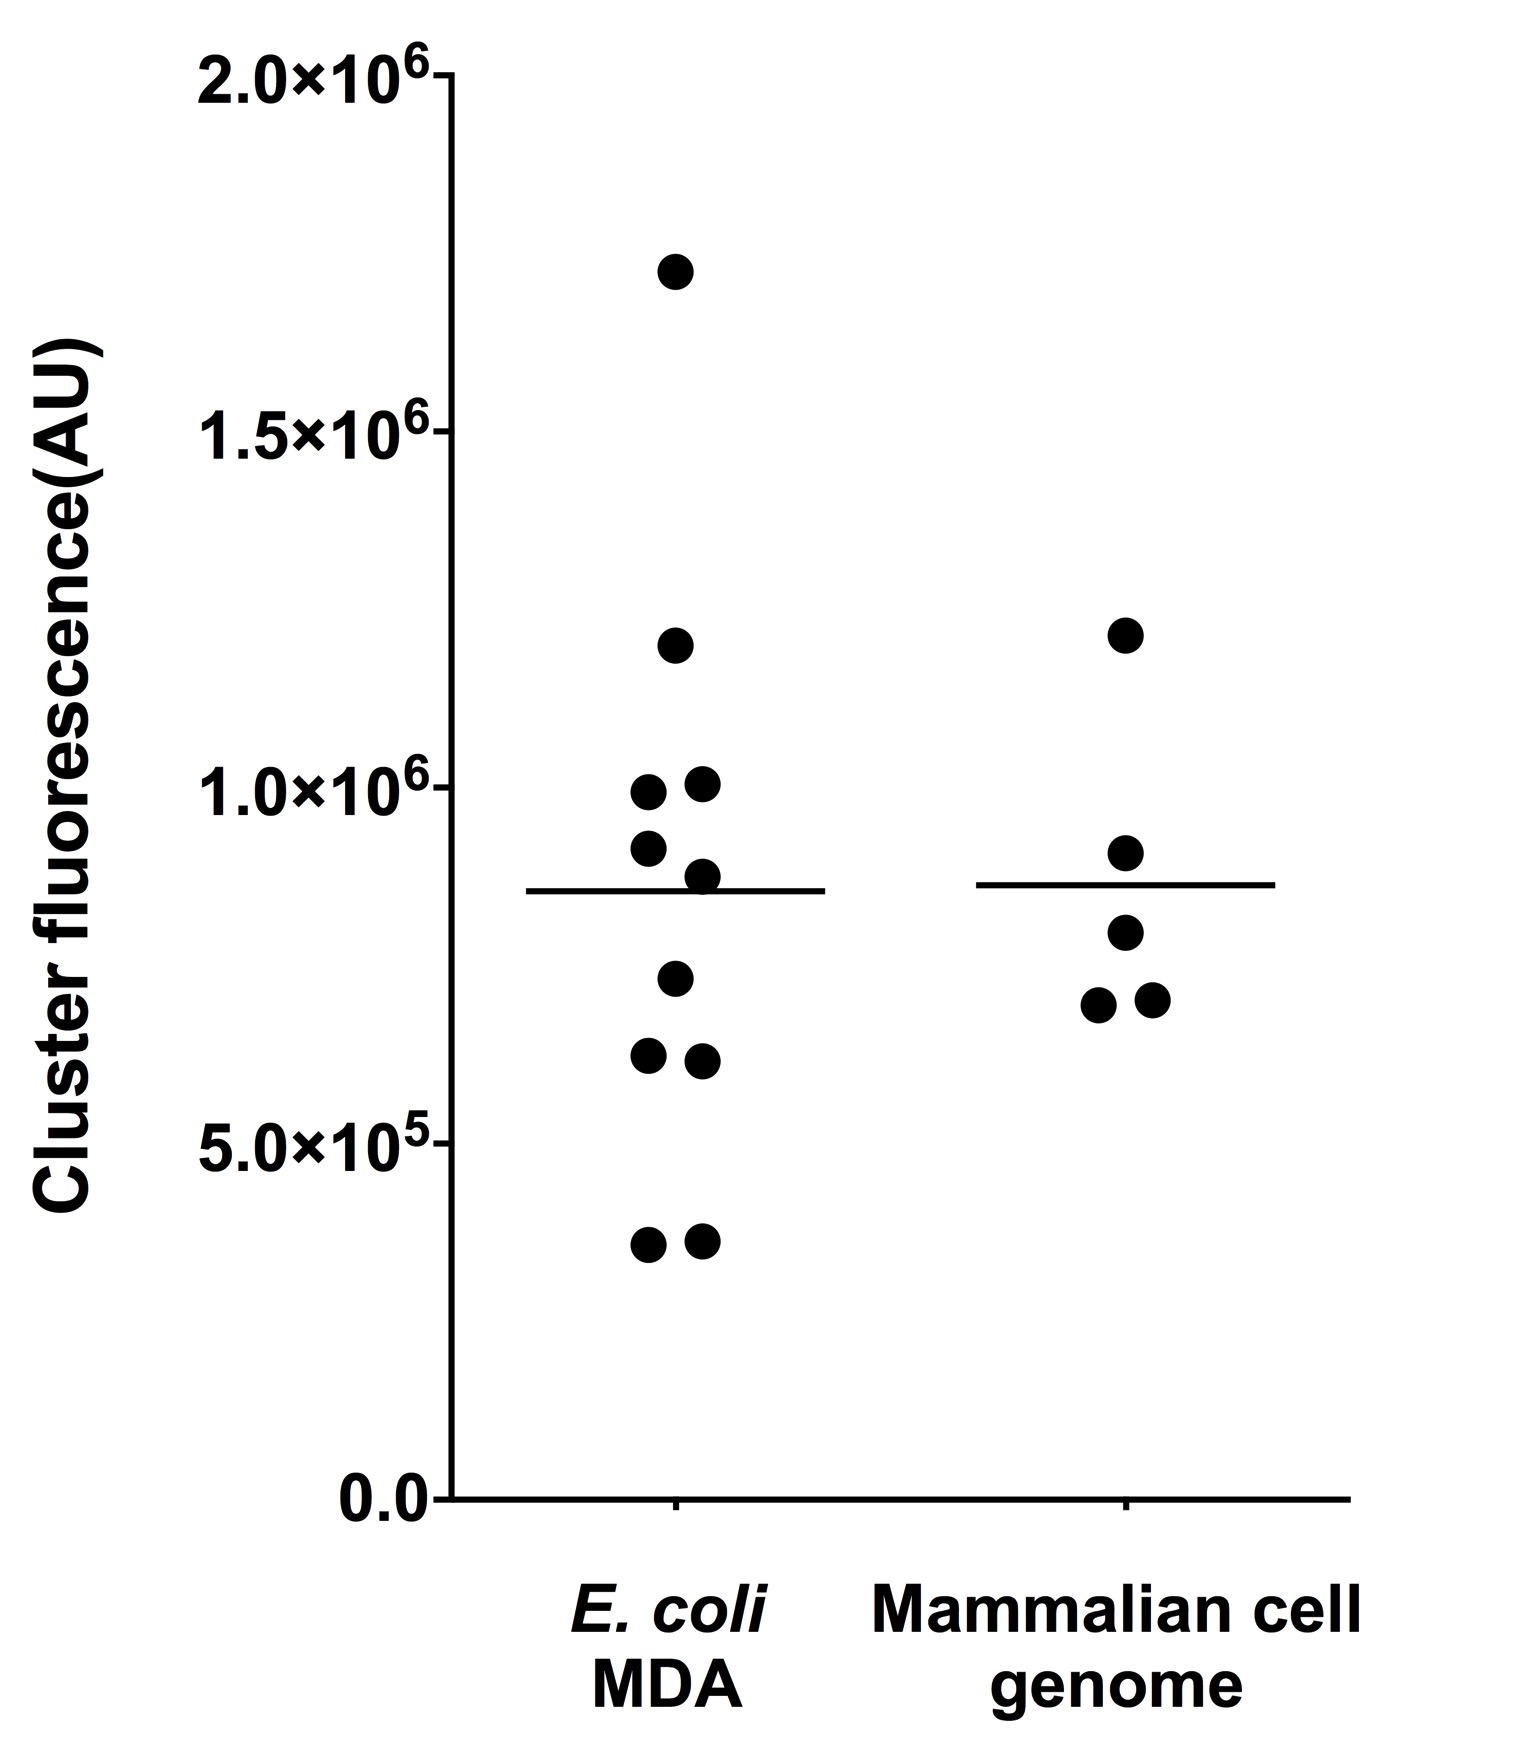
\includegraphics[keepaspectratio,width=0.5\textwidth]{./figures/SuppFig2.jpg}
% \caption[\textit{E. coli} MDA cluster quantification.]{\textit{E. coli} MDA cluster quantification. \textit{E. coli} MDA cluster's DNA content was calibrated against (unamplified) hydrogel-embedded mammalian cells (HEK 293) by comparing SYTOX Orange fluorescence intensities. DNA content in individual product clusters and mammalian cells was approximated by integrating pixel intensities under the same hydrogel and staining conditions. The observed integrated fluorescence was comparable across MDA product clusters and unamplified mammalian cells, leading us to conclude that the average DNA content per MDA product cluster was approximately equal to the average DNA content of an unsynchronized mammalian cell population, or on the order of 10 pg. The centerline represents the mean value.}
% \label{fig:SuppFig2}
% \end{figure}

\subsection{Image acquisition and analysis}
Z-stack images were taken by Nikon ultra-fast laser scanning confocal microscope with pinhole = 1.2, HV = 112, offset = 0, laser wavelength = 561 nm, laser power = 1.3 to 1.5, using a 20$\times$ objective on Galvano mode. Acquisition speed was 1 frame\slash sec and z step size was 0.95 $\mu$m. On the inverted microscope, z-stack images were taken with the exposure time 100 ms, Lumencor excitation power 10\%, binning size 2 and z step size 10 $\mu$m. Both z stacks were first processed into max intensity projections in FIJI. Max projection tiff files were then loaded into MATLAB. The background was obtained by applying a Gaussian filter of hsize 200 and sigma 50. All max projections were background-subtracted and thresholded at 2 $\sim$ 2.5$\times$ standard deviations above the mean intensity. Cluster count, cluster area (radius), and cluster mean intensity were obtained with the bwconncomp and regionprops functions (Fig. \ref{fig:dMDA_MammalianEcoliCluster}).

\begin{figure}
\centering

\includegraphics[keepaspectratio,width=1\textwidth]{./figures/MammalianEcoliCluster}
\caption[Imaging analysis for a \textit{E. coli} MDA cluster and a mammalian genome]{Imaging analysis for a \textit{E. coli} MDA cluster and a mammalian genome. a) The \textit{E. coli} MDA cluster and the mammalian genome were imaged with a Nikon confocal microscope. The cluster radius of each were ploted. b) The mean fluorescence of each stack was plotted for the \textit{E. coli} MDA cluster and the mammalian genome.}
\label{fig:dMDA_MammalianEcoliCluster}
\end{figure}